\chapter{The biotic and abotic mechanisms of patch size response}
\label{chap:astar}

\subsection{Introduction}\label{introduction}

Many ecological communities exist across patchy habitats. In such
communities, not all species are found in all patches -- some are
present in only large patches, some only in small patches, others show a
weak relationship to patch size \citep{Taylor1991, Lomolino2000}. This
variation in patch size response has important community-level
consequences. For example, preference for different patch sizes may
facilitate coexistence among similar species \citep{Gilbert2008}.
Variation among individual species in their response to patch size also
underlies the species-area relationship \citep{Ovaskainen2003}. Although
such variation in response to patch size is common in nature, we know
little about what creates this variation. Part of the challenge is that
species' response to patch size is determined by at least three
different covariates of patch size: numerical effects, abiotic
variation, and species interactions. To understand how species are
distributed across patches, we need to first measure the extent to which
each of these processes varies with patch size.

Some of the variation in species occurrence across patches is caused by
numerical effects. Numerical effects are the combined result of two
phenomena: species differences in relative abundance (at the scale of
the metacommunity), and patch differences in capacity (at the level of a
local patch within the metacommunity). Rare species are more likely
occur in larger patches, because larger patches contain more individuals
\citep{Wright1991}. Common species are also more likely to occur in
larger patches, as larger patches may also sustain larger populations,
which in turn decreases demographic stochasticity -- making common
species more likely to persist. These mechanisms do not depend upon any
specific traits of species (i.e.~are stochastic with respect to traits
\citep{Vellend2014}). Rare species might appear to prefer larger
patches, but this preference disappears when compared to the correct
null model \citep{Srivastava2008}. Therefore, when studying the
distribution of organisms along a patch size gradient, the first step is
to estimate the numerical effects associated with patch capacity and
relative abundance.

Species occurrence in larger patches may also depend on the abiotic
effects with covary with patch size. Larger habitat patches may be more
environmentally stable -- for example, microclimatic variables in forest
patches are often less variable than smaller fragments
\citep{Matlack1993}. Larger patches may also be more productive (for
example in the case of islands \citep{Schoener1989}); this can increase
the number of individuals and therefore the number of species per island
\citep{Wylie1993, Kalmar2006}. Larger patches may have a decreased risk
of disturbance, though this depends on the system. For example, small
Caribbean islands are often also lowlying, and thus are frequently
inundated by hurricanes \citep{Schoener2001}. In contrast, large
temperate islands are more frequently hit by lightening
\citep{Wardle1997}. These qualities of large patches can affect the
probability that a given species will colonize and establish in a patch.

Although numerical effects and abiotic factors can directly determine
how a focal species responds to patch size, such factors may also
indirectly determine the response of a focal species by changing the
surrounding food web. Some species in this food web, such as competitors
and often predators, can reduce the persistence of the focal species;
other species, such as facilitators and even predators (in case of
predator-mediated coexistence \citep{Caswell1978}), can have the
opposite effect. If we focus for the moment just on negative species
interactions, indirect effects of patch size may have a myriad of
effects on species incidence. If larger patches have more species of
competitors and predators (through either numerical or abiotic effects),
then larger patches may be more likely to contain a particular
antagonistic species, reducing the incidence of a focal species in such
patches. For example, lizards are more common in large glades in the
Ozarks (southern USA), causing their preferred prey - grasshoppers and
spiders - to occur disproportionately in small glades
\citep{Ostman2007, Ryberg2007}. On the other hand, the high species
diversity in large patches may in itself stabilize populations. Speciose
communities may have more diffuse competitive and trophic interactions;
such interactions have been shown to stabilize populations
\citep{Aschehoug2015, Rooney2006}, potentially increasing the incidence
of our focal species in larger patches.

In any species-rich community, we expect there to be variation among
species in the role of numerical, abiotic and biotic processes
underlying species' responses to patch size. Each of these processes may
have a phylogenetic signal, if conserved traits of species determine
relative abundance (numerical effects), their environmental tolerances
(abiotic effects) and their interspecific interactions (biotic effects).
This phylogenetic signal, however, may result in closely related species
either converging or diverging their response to patch size. When
numerical and abiotic processes dominate, we would expect closely
related species to be similarly sensitive to patch size because they
share the traits that determine abundance (e.g.~intrinsic growth rates),
environmental tolerance (e.g.~drought resistance), or both. However,
when biotic processes dominate, similarity in response between related
species may depend on the precise type of species interaction being
considered. For example, when closely related prey species share traits
that determine predator resistance \citep{Nyman2007}, they may both
occur in patches where predators are absent. If predators are more
common in larger patches, this would cause a similar patch size response
(caused by predators) in both prey species. On the other hand, when
closely related species share traits related to resource acquisition,
intense competition may result, thereby reducing the likelihood of local
co-occurrence \citep{Webb2002}. If resource availability is related to
patch size, regional coexistence of such species may be possible when
each species is the superior competitor within a different range of
patch size. Similarly, where predation risk changes with patch size,
trade-offs between predation resistance and competitive ability could
also result in different patch size associations of closely related
species.

\begin{figure}[htbp]
\centering
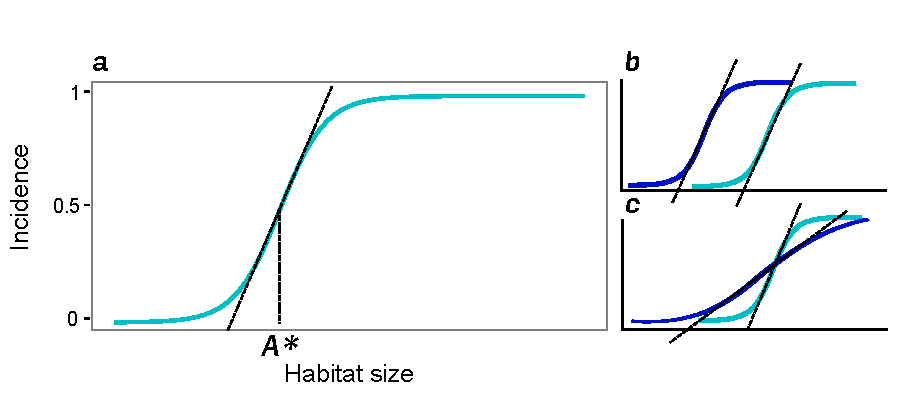
\includegraphics[width=5.5in]{figures/illustration.pdf}
\caption[Conceptual diagram of incidence functions]{Incidence functions (\textbf{a}) estimate the probability of
occurrence of a species (y-axis) as a function of patch size. These
functions can be estimated using logistic regression, and can be
parameterized with two values: \(A^{*}\) (The position of the inflection
point) and \(x\) (the slope at the inflection point). Species can differ
in either of these parameters: in \textbf{b}, two species differ in
their \(A^{*}\) value, and in \textbf{c} they differ in \(x\).}
\label{fig:concept}
\end{figure}

Variation in response to patch size can be quantified with incidence
functions. Incidence functions describe how the occurrence, or
incidence, of a species changes over a gradient of patch size. This
use of incidence functions originated with the study of birds on
tropical islands \citep{Diamond1986} and has been extended to predicting
parameters of the species-area relationship \citep{Ovaskainen2003}. The
incidence function is usually modeled as a logistic relationship between
the probability of encountering a species and habitat area. These
S-shaped curves can be described by two parameters: \(A^{*}\), the size
at which there is a 50\% chance of a species occurring, and \(x\), which
is proportional to the slope of the curve at that value (Figure \ref{fig:concept}). In
other words, \(A^{*}\) describes the threshold size of patch in which a
species is found, and \(x\) describes the strength of patch size
preference. These two ways of expressing response to area give us a
means to understand how species coexist along a patch size gradient.
Coexistence may be promoted in two ways: species may partition the size
gradient (different \(A^{*}\) values), or species may form a
generalist-specialist pair (low and high \(x\) values respectively). Partitioning
of habitat gradients in general has been related to the coexistence of
species, with well-known examples including sticklebacks
\citep{Rundle2000}, warblers \citep{MacArthur1958}, and annual plants
\citep{Seabloom2003}. Similarly, many species coexist in
specialist-generalist pairs along habitat gradients. For example, two
coexisting parasitoids coexist because one, the inferior competitor, can
survive on less productive host populations \citep{Amarasekare2000}.
Likewise, in \emph{Eutamias} chipmunks, two species coexist on an
altitude gradient, with the inferior competitor limited to higher, less
productive elevations \citep{Sheppard1971}.

We tested three hypotheses related to patch size response. First, using
observational data, we account for numerical effects and test three
hypotheses about community-level patterns: (1) there is more variation among species
in patch size response than expected by chance. (2) species pairs are divergent in
both their critical size threshold (\(A^{*}\) value) and the strength of
preferences (\(x\) value). (3) that this divergence in patch size
response is greater for close relatives. We then use an experiment to
test three hypotheses about species-level processes causing this between-species variation: (4) species trade off their ability to tolerate
environmental conditions associated with different patch sizes with
their ability to withstand either competition or predation. (5)
competition alone limits the distribution of species along a gradient of
patch sizes, or (6) predation alone limits the distribution of species
along a gradient of patch sizes.

\subsection{Methods}\label{methods}

\subsubsection{Study system}\label{study-system}

Bromeliads offer a useful system in which to study the effects of
patch size on species occurrence. Bromeliads (Bromeliaceae) are
flowering plants found throughout the Neotropics. Many members of the
family form ``tanks'' in their leaf wells, which collect rainwater and
detritus. This phytotelmata is the habitat for a community of
specialized animals \citep{Frank2009, Benzing2000}. The insect community
contains a large number of species, which are diverse in taxonomy and
trophic positions. This aquatic habitat is naturally patchy, and patches
vary widely in volume (our measure of size) by several orders of
magnitude, ranging from very small (10s of ml) to quite large
(\textasciitilde{}4000 ml). This gradient of size correlates with a
large number of abiotic and biotic factors, including: drought risk
\citep{Amundrud2015}; habitat complexity \citep{Srivastava2006a}; algal
productivity \citep{Marino2011}; detrital density
\citep{Richardson1999}; and potentially, although undocumented, water
chemistry. The gradient of size is present at different spatial scales:
larger plants also have larger leaf wells. Some of these abiotic
variables can also affect species interactions. Habitat complexity
affects the efficiency of predators \citep{Srivastava2006a}, whereas
detritus and algae represent resources for many macroinvertebrates
(Farjalla et al. 2016). The ease with which bromeliads are sampled and
manipulated makes them ideal systems for investigating differences
between coexisting species in response to patch size. Both
observations and experiments were conducted in Parque Estadual da Ilha
do Cardoso (25\textsuperscript{o} 03' S, 47\textsuperscript{o} 53' W), a
22.5 ha island off the south coast of São Paulo state, Brazil. We worked
in a coastal forest (\emph{restinga}) with an understory dominated by
\emph{Quesnelia arvensis} Mez. (Bromeliaceae).

\subsubsection{Quantifying species variation in response to patch
size}\label{quantifying-species-variation-in-response-to-patch-size}

To quantify how species vary in response to patch size, we surveyed
bromeliads of different size. In 2008 we collected 30 bromeliads,
dissected them, and collected the macroinvertebrates. “Size” is defined here as a bromeliad’s maximum water-holding capacity; these bromeliads
were chosen to equally distribute their maximum capacity on a logarithmic
scale. Maximum capacity has been shown in other
studies to be superior to other potential size metrics in predicting
bromeliad invertebrate communities \citep{Srivastava2008, Marino2011}.
We measured maximum volume by emptying a bromeliad, then pouring a known
volume of water into the bromeliad and subtracting the overflow.

\paragraph{(1) Community-level variation in patch size
response}\label{community-level-variation-in-patch-size-response}

To quantify variation in size response we calculated an unbiased
measurement of average pairwise differences in species responses, which
requires two steps: first, estimating average difference between species
in patch size response from data, and second, comparing this community
average to a null model. \textbf{Step 1:} We modelled the presence of
invertebrate species as a logistic function of maximum plant volume (log
transformed). We calculated two parameters from these logistic curves: as the inflection point -- the
``\(A^{*}\) value'' -- and \(x\), the slope of the linear predictor
\citep{Ovaskainen2003}. The ``\(A^{*}\) value'' corresponds to the plant
volume with a 50\% chance of species occurrence (i.e.~the inflection
point of a logistic curve). For every pair of species we quantified the
pairwise difference in their parameter estimates, as the absolute
difference in estimates divided by the square root of summed squared
standard errors:

\[D_{b_{ij}} = \frac{|b_{i} - b_{j}|}{\sqrt{SE_{b_{i}}^{2} + SE_{b_{j}}^{2}}}\]

Where \(b\) is the parameter estimate (either \(A^{*}\) or \(x\)) for
each species (\(i\) and \(j\)) in a pair. We estimated \(x\) as the
slope of the linear predictor in logistic regression, and \(A^{*}\) as
the inflection point of the logistic curve (calculated with
\texttt{dose.p} from the package MASS \citep{mass}).

We calculated the average patch size response as the average difference
between all pairs of species in their \(D_{b_{ij}}\) values (i.e.~we repeated this calculation once for \(A^{*}\) and again for \(x\)).

\textbf{Step 2:} Species abundances can create spurious patterns in measurements of
patch size response; we therefore used a null model to create an
unbiased estimate of pairwise \(D_{b_{ij}}\). In each null simulation,
we randomly shuffled individual invertebrates among bromeliads, stopping
when a bromeliad contained the same number of individuals as in our
observation. This approach therefore maintains both the total number of
individuals in each species (fixed across all simulations), and the
total number of individuals in each bromeliad (fixed across all
simulations). The resulting simulations contain only the effects of
bromeliad size on species composition -- that is, it removes any
species-specific preference for a particular bromeliad size, and any
pattern of association between species \citep{Ulrich2012}. This null
model is necessary because sampling effects can create large values of
\(D_{b_{ij}}\). For example, rare species tend to have a higher observed
\(A^{*}\) value, merely because they are more likely to be found in a
large bromeliad with high abundance \citep{Srivastava2008}. We repeated
this randomization 999 times. For every null simulation we re-calculated
the values of \(D_{b_{ij}}\) for both \(A^{*}\) and \(x\), for all
species pairs. We then averaged all \(D_{b_{ij}}\) within each
simulation, creating a null distribution of community-level values of
\(A^{*}\) and \(x\) (999 values each). We calculated the standardized
effect size (SES) of the observed mean against this null distribution:

\[SES_{D} = \frac{D_{obs} - \bar{D}_{null}}{SD_{null}}\]

where \(\bar{D}_{null}\) is the mean of all null \(D_{b_{ij}}\) values
and \(SD_{null}\) is the standard deviation of that that null
distribution. We calculated a null p-value as the proportion of
simulations that were more extreme than our observed \(D_{b_{ij}}\)
value for each parameter.

\paragraph{(2) Divergence between species pairs in patch size
response}\label{divergence-between-species-pairs-in-patch-size-response}

We followed a similar approach to standardize the patch size response of
individual species pairs. Rather than averaging all pairwise differences
to create a single community average, we compared each observed pairwise
difference between species to those calculated under the null
simulations. We once again calculated \(SES_{D}\) for both \(A^{*}\) and
\(x\), this time for each species pair. Because differences in patch
size response between species are partly caused by numerical effects,
these \(SES_{D}\) represent unbiased estimates of how different two
species are in the way they respond to patch size.

\paragraph{(3) Do close relatives show more similar, or more different,
size
responses?}\label{do-close-relatives-show-more-similar-or-more-different-size-responses}

Finally we tested the hypothesis that variation \(SES_{D}\) is
correlated with the taxonomic relatedness of a species pair. We grouped
pairs of species into three taxonomic groups, depending on the lowest
taxonomic rank they share: pairs of species in the same Order, Family
and Genus. We tested the hypothesis that similarity in relatedness
increases \(SES_{D}\), with a linear regression of \(SES_{D}\) as a
function of the taxonomic rank of each pair. Because these points are
not independent (i.e.~the same species can occur in multiple pairs), we
then tested the significance of this linear contrast with a
randomization test, by randomly permuting the taxonomic groups 999
times.

\subsubsection{Causes of different size responses -- field
experiment}\label{causes-of-different-size-responses-field-experiment}

If a pair of taxa -- even close relatives -- show significant
\(SES_{D}\), this indicates that processes other than numerical effects
are driving this variation. Do these species respond differently to
environmental variation (i.e.~to patch size itself) or to species
interactions (presence of competitors and predators) or both? We chose
one such species pair for our experiment: \emph{Polypedilum kaingang}
and \emph{Polypedilum marcondesi} (Diptera: Chironomidae). We contrasted
the performance (combined survival and emergence) of these two
congeneric chironomids. This is a particularly interesting species pair,
as \emph{P. kaingang} is a patch size generalist whereas \emph{P.
marcondesi} occurs disproportionately in large bromeliads.

To measure the effect of the abiotic gradient, we transplanted these two
species of \emph{Polypedilum} species across this bromeliad size
gradient. We found 10 bromeliads which were larger and 10 smaller than
the size threshold for the two \emph{Polypedilum} species, which we
estimated as 500ml. In order to determine the volume of these plants
without disturbing their insect community, we used allometric equations
based on the number of leaves: plants with \textless{} 35 leaves were
categorized as ``small'', plants with \textgreater{} 45 leaves as
``large''. We used plastic centrifuge tubes to create controlled
environments within each leaf well. Tube sizes were chosen to imitate
the approximate volume of a leaf well: 15 ml tubes for small plants, and
50 ml tubes for large plants. In each bromeliad, we placed 4 plastic
centrifuge tubes (see below) in randomly chosen leaf wells within each
bromeliad.

To measure the effect of the biotic gradient (presence of competitors
and predators) each of the 4 tubes in each bromeliad received one of
four ``community treatments''. These treatments were chosen to measure
the effect of predators and competitors on these two species of
\emph{Polypedilum}. We used two ``alone'' treaments, 5 individuals
\emph{P. marcondesi} or 5 individuals \emph{P. kaingang}; one
``competition'' treatment, both species together (10 individuals total);
and one ``competition and predation'' treatment -- both together with a
predator (a damselfly larvae, \emph{Leptagrion elongatum}). Each
bromeliad (small or large) received all treatments (n = 10 bromeliads
per treatment).

We attempted to create experimental tubes that mimicked the abiotic
conditions of a natural leaf as closely as possible. We randomly
selected water-filled leaves within each experimental bromeliad. We
collected the water and thoroughly removed all visible
macroinvertebrates, then allowed the water and detritus to sit in the
lab for a minimum of 12 hours before searching again. This allowed any
animals which were in early stages (eggs or larvae) to be removed. In
order to preserve the community of the leaf well as much as possible
(e.g.~bacterial communities, particle size distribution of detritus,
etc), we did not filter this water. We transferred this water to an
experimental tube, which was placed deep in the original leaf well.
Tubes isolated the water from the bromeliad environment, but had tubes
with large holes in the side, covered with Nytex™ mesh (0.5mm). The mesh
let water flow into the tube from the bromeliad, maintaining the water
chemistry within the tube. The tubes were also capped with a mesh bag,
which allowed us to capture emerging adults.

We measured performance of each species by recording the emerged adults
each day for 60 days. We also counted surviving larvae at the end of the
experiment; the sum of emerged adults and surviving larvae is our
measure of performance.

We analyzed performance of each species with a linear mixed-effects
model, after log transforming the performance response. We included
treatment (each species alone, with a competitor, or with a competitor
and a predator) and bromeliad size as fixed factors, and bromeliad
identity as a random factor. We fit these models using the lmerTest
package \citep{lmertest} in the R statistical language \citep{rcore}. We
defined \emph{a priori} contrasts to test specific hypotheses about the
effects of different factors on chironomid performance. To quantify the
effect of predators on performance, we contrasted our predator and
competitor treatment with the competitor-only treatment (``predator
absent'' contrast). To quantify the effect of competitors, we contrasted
the mean of both treatments with competitors (with and without
predators) with the control treatment (no competitors or predators).
This was our ``competitor absent'' treatment.

\subsubsection{Figures}\label{figures}

\begin{figure}[htbp]
\centering
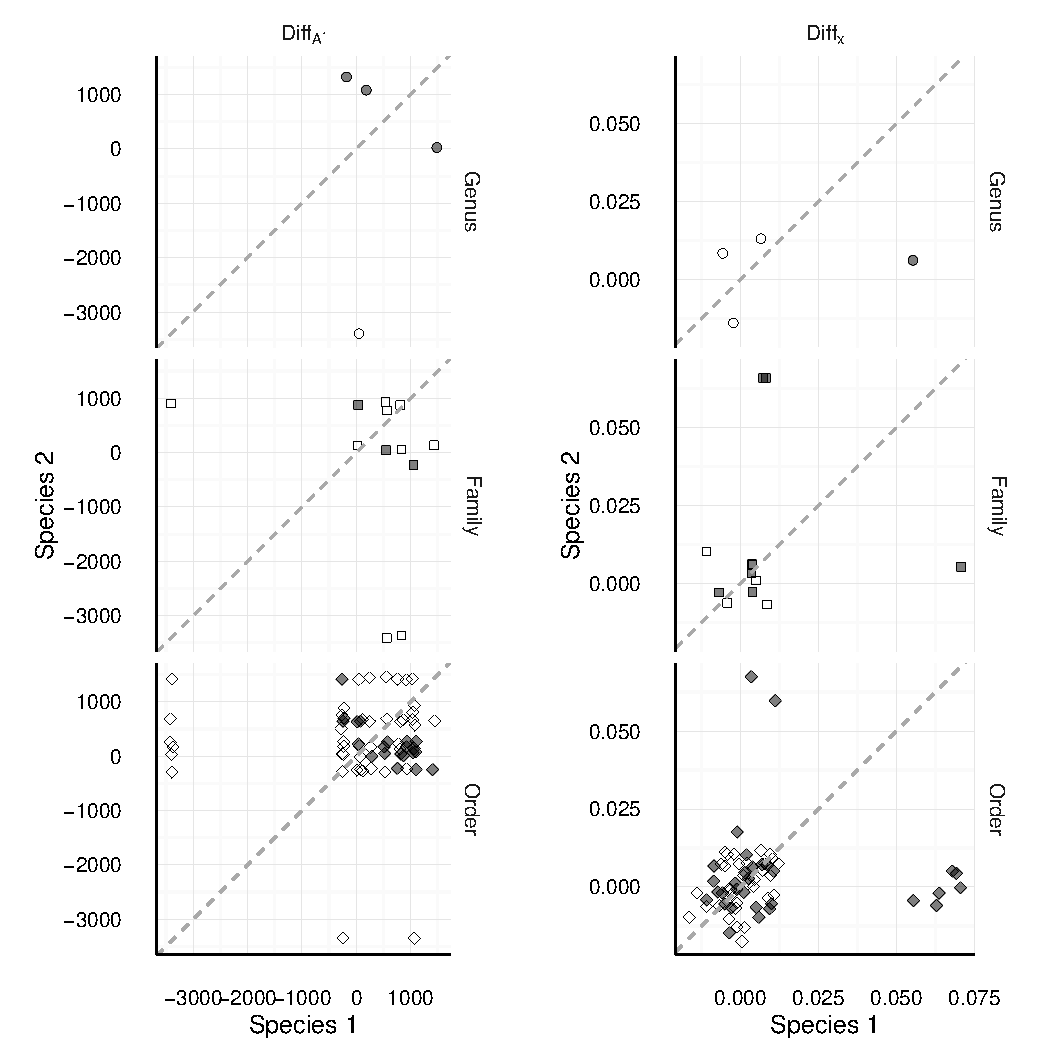
\includegraphics[width=5.5in]{figures/pairwise_astars.pdf}
\caption{Pairwise differences in two measures of size response. Each point represents a
pair of species, divided into species pairs within the same genus (top)
the same family (middle) and order (bottom). The left panel shows
differences in \(A^{*}\) values (units are ml) while the right panel
shows differences in \(x\) (slopes of logistic regression). Species
pairs which are different from a null model are shaded.}
\end{figure}

\begin{figure}[htbp]
\centering
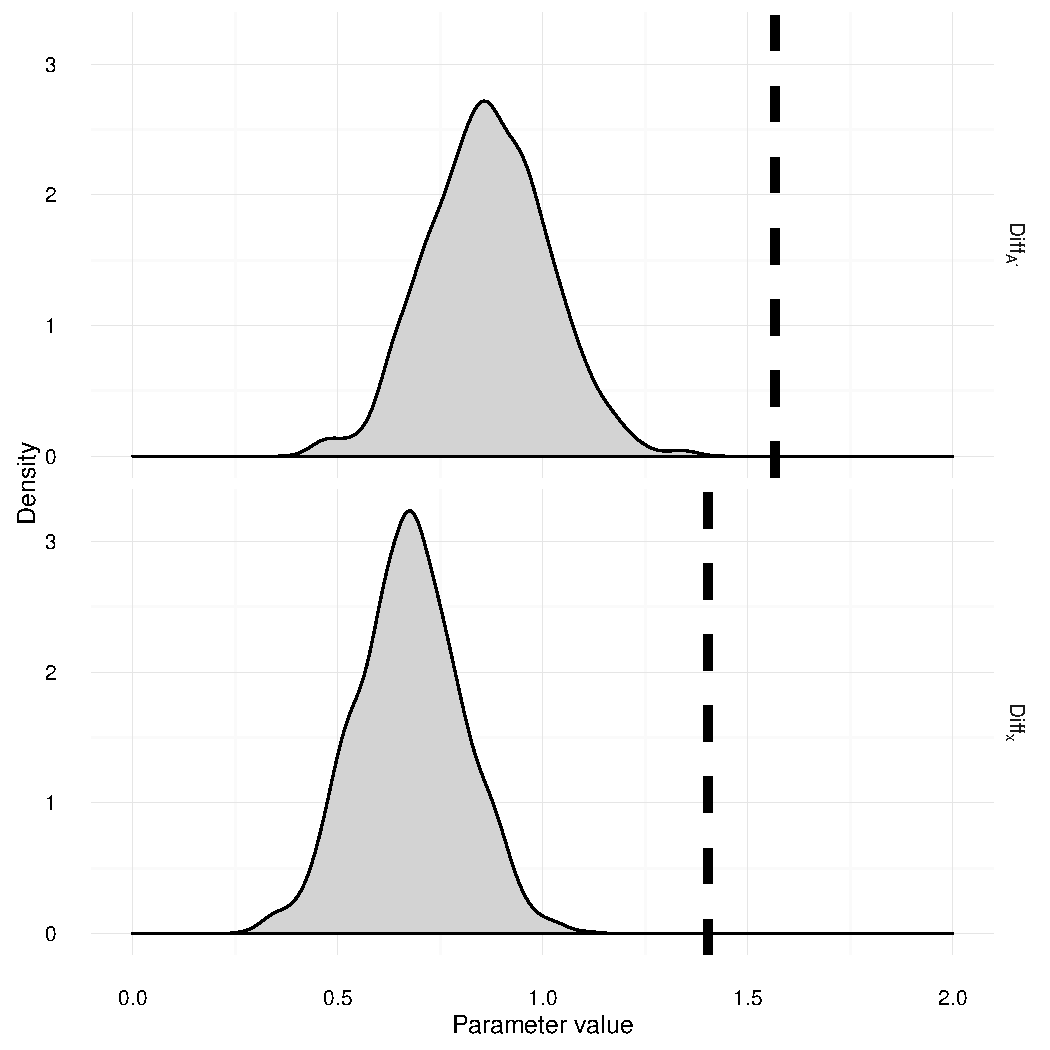
\includegraphics[width=5.5in]{figures/overall_null.pdf}
\caption{Mean pairwise
differences between species in two measures of patch size responses:
patch size threshold (\(A^{*}\)) and strength of patch size preference
(\(x\)). Dashed vertical lines represent observed means for all species
pairs. Grey histograms represent means for 999 null simulations.}
\end{figure}

\begin{figure}[htbp]
\centering
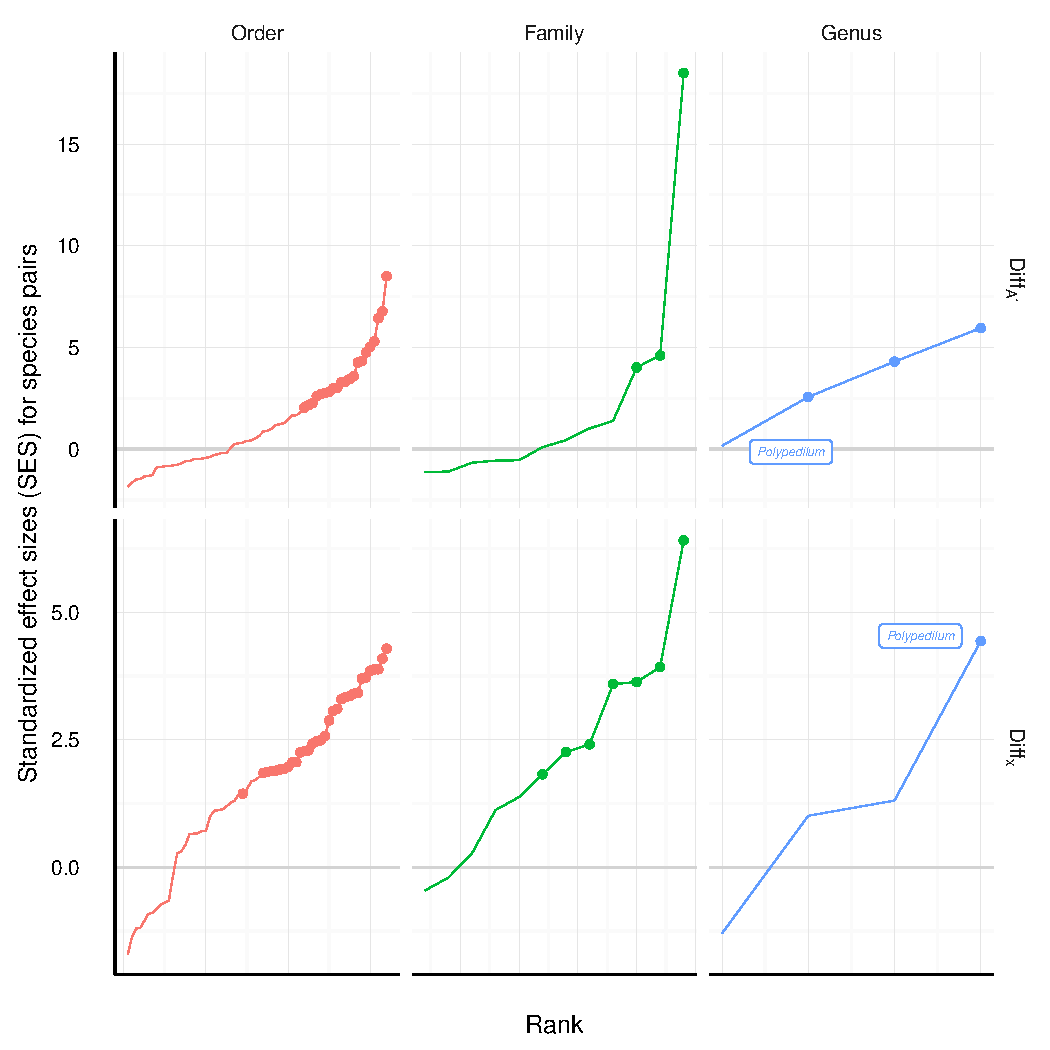
\includegraphics[width=5.5in]{figures/ses_rank.pdf}
\caption{Standardized effect sizes (SES) of pairwise differences
between species for two different measures of patch size response.
These two measures are critical patch size (\(A^{*}\)) and strength of
patch size dependency (\(x\)). Pairwise differences are shown within
each of three taxonomic levels. Significant standardized effect sizes
(randomization p-value \textless{} 0.05) are indicated with points.}
\end{figure}

\begin{figure}[htbp]
\centering
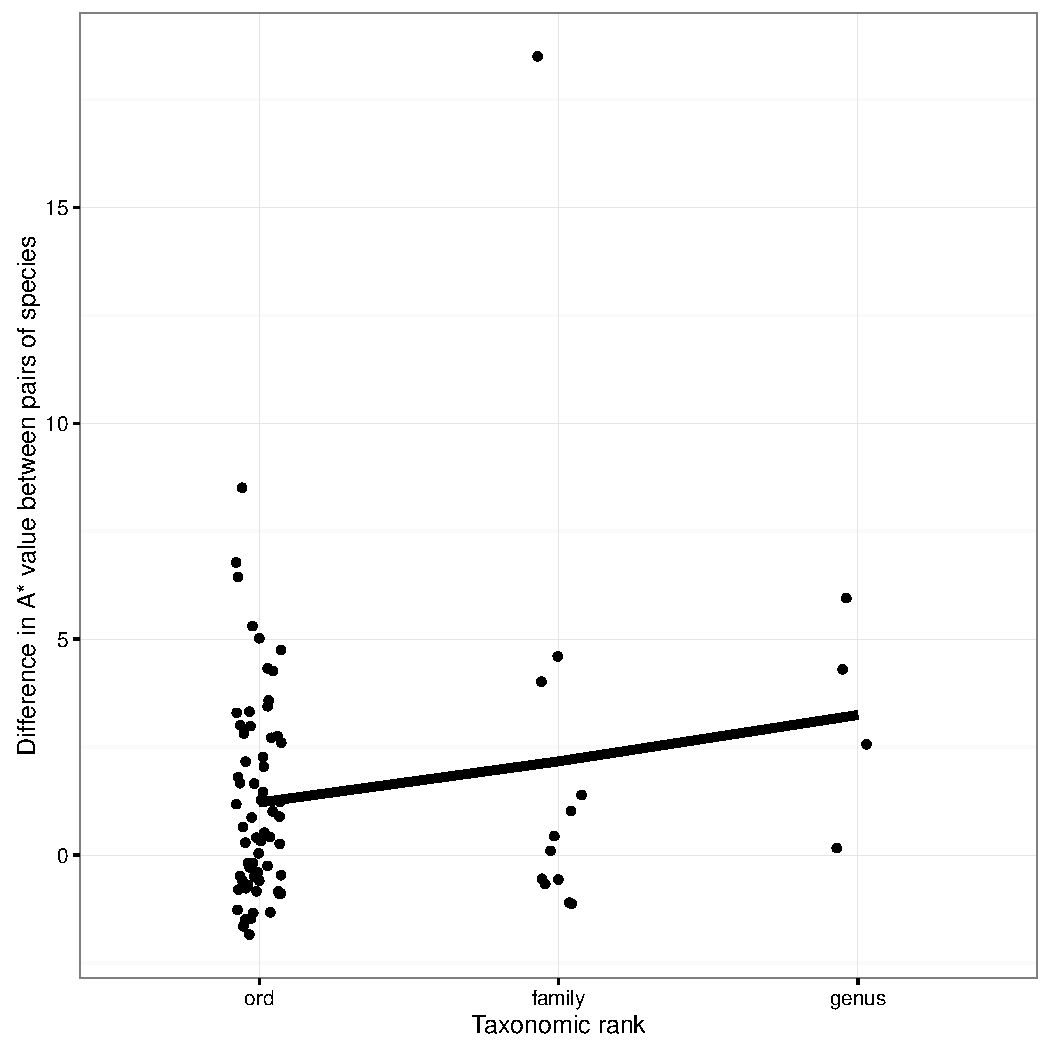
\includegraphics[width=5.5in]{figures/astar.pdf}
\caption{Differences in observed
threshold patch size (\(A^{*}\)) increases with taxonomic similarity
of species pairs, measured as the lowest taxonomic rank in common
between two species (black line connects observed means of each
taxonomic rank).}
\end{figure}

\begin{figure}[htbp]
\centering
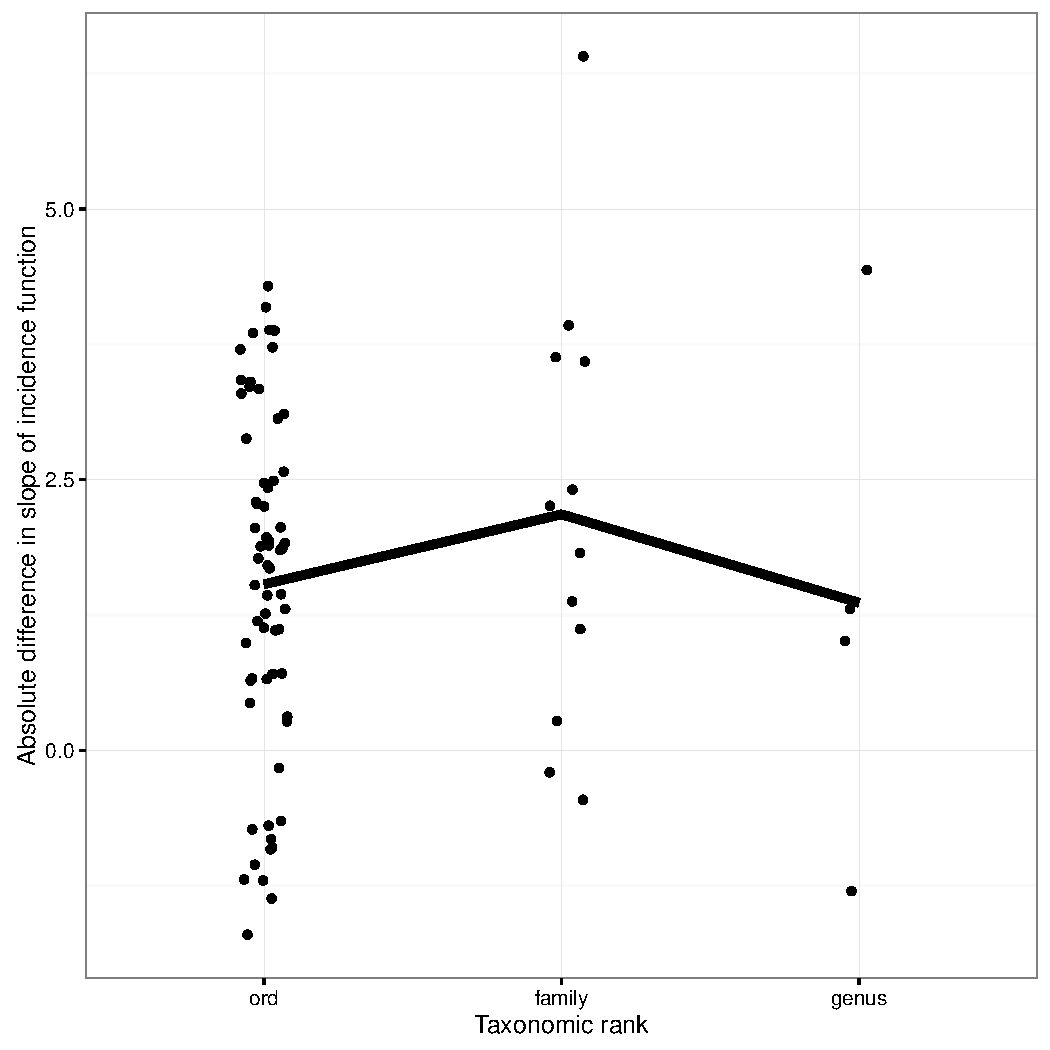
\includegraphics[width=5.5in]{figures/xbar.pdf}
\caption{Differences in (\(x\)) between pairs of species, as a function of
their taxonomic similarity, measured as the lowest taxonomic rank in
common between the two species. (\(x\)) measures
the slope of the incidence function. Black dots indicate observed
species pairs; black line connects means of observed values. We observed
no relationship between differences and taxonomic relatedness.}
\end{figure}

\begin{figure}[htbp]
\centering
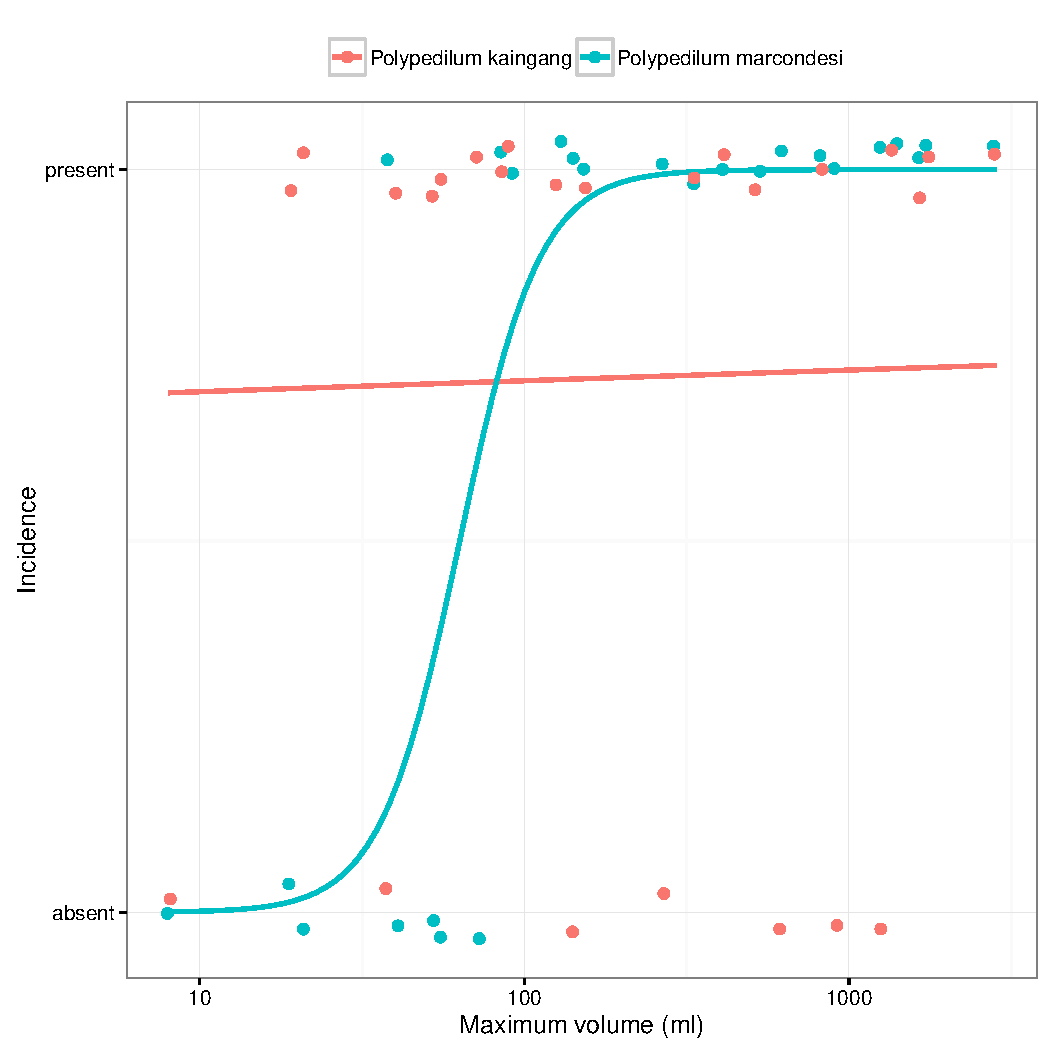
\includegraphics[width=5.5in]{figures/poly_curve.pdf}
\caption[\emph{Polypedilum marcondesi} is a patch size specialist occurring
only in large plants. \emph{Polypedilum kaingang} is found across the
gradient of bromeliad size.]{Two closely
related species that show very different responses to patch size.
\emph{Polypedilum marcondesi} is a patch size specialist occurring
only in large plants. \emph{Polypedilum kaingang} is found across the
gradient of bromeliad size. Note logarithmic x-axis scale.}
\end{figure}


\begin{figure}[htbp]
\centering
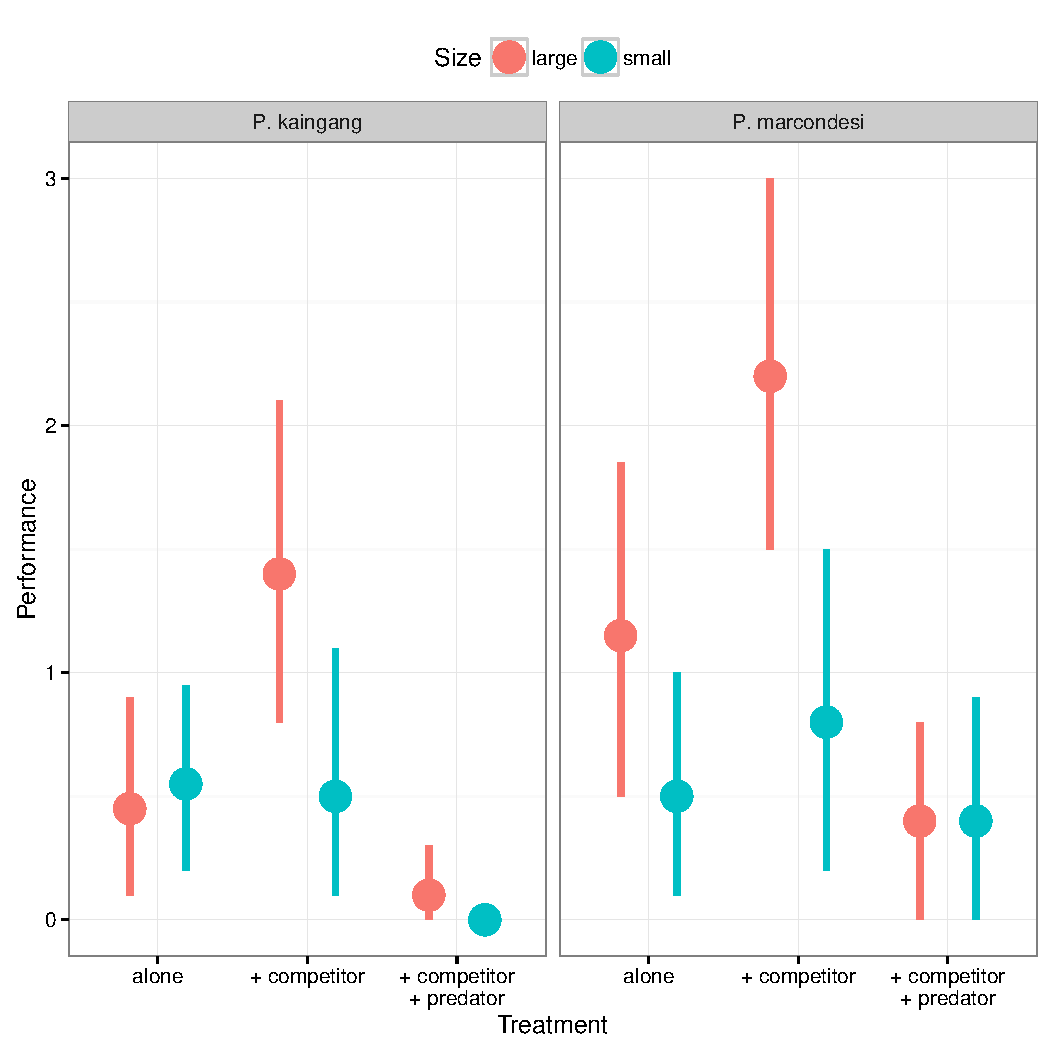
\includegraphics[width=5.5in]{figures/anova_data.pdf}
\caption[Performance (larvae + emergences) of \emph{P. marcondesi} and
\emph{P. kaingang}.]{Performance (larvae + emergences) of \emph{P. marcondesi} and
\emph{P. kaingang} across all biotic treatments.}
\end{figure}

\begin{figure}[htbp]
\centering
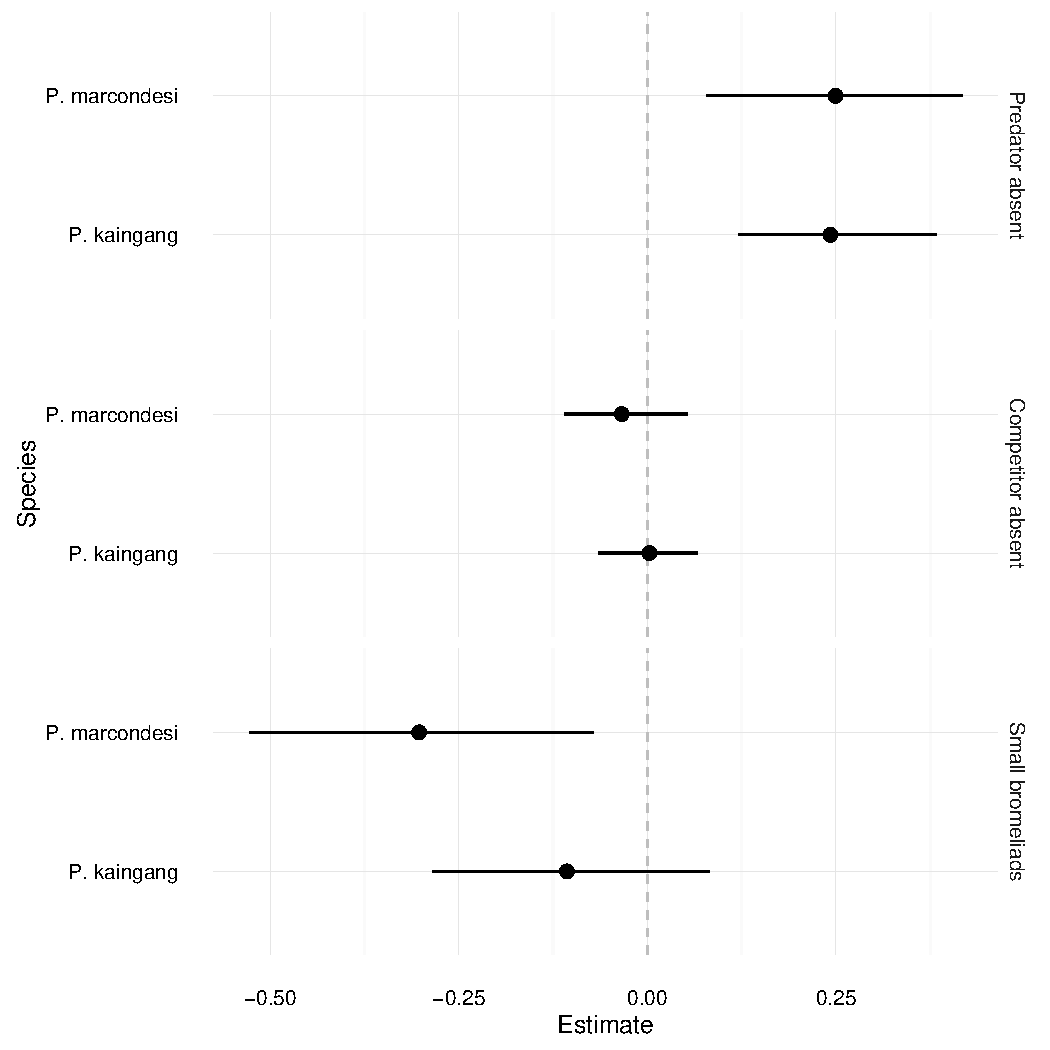
\includegraphics[width=5.5in]{figures/confints.pdf}
\caption[Small bromeliads reduce \emph{P. marcondesi} performance.]{Small bromeliads reduce \emph{P. marcondesi} performance. Points give the mean and 95\% confidence intervals for our \emph{a priori} contrasts between our treatment levels. The absence of predators increases prey emergence, while the presence of competitors had no effect.}
\end{figure}


\subsection{Results}\label{results}

We observed 21 morphospecies of aquatic larvae in the 2008 survey, of
which 17 could be identified enough for our taxonomic analysis (Figure
2). On average, pairs of species were more divergent in their response
to patch size than would be expected by simple numerical effects,
whether we considered threshold patch size (\(A^{*}\), Figure 2) or the
strength of patch size preference (\(x\), Figure 2). Specifically, we
found that all taxa were either equal or divergent in these two measures
of their response to patch size (i.e.~there were no negative
standardized effect sizes, Figure 4).

\subsubsection{Observed patch size differences and taxonomic
relatedness}\label{observed-habitat-size-differences-and-taxonomic-relatedness}

Taxa that were more closely related tended to differ more in their size
thresholds (\(A^{*}\) values) than more distantly related taxa (slope =
0.99, Figure 5). Null models predict the opposite relationship: based
just on numerical effects, taxa that are more closely related tend to
differ less in their size thresholds (linear contrast from ANOVA, mean $\pm$
sd 0.017 $\pm$ 0.66). Comparing the actual with null model pattern, we can
conclude that observed species pairs (especially congenerics) had
greater differences in critical size than expected from variation in
relative abundance alone but that this difference was marginally
insignificant (SES of observed slope, 1.48, p = 0.0851, Figure 5).

Taxa that were more closely related tended to be more similar in the
strength of their preference for patch size (slope, 0.2 Figure 6).
This does not differ from the null expectation (Average of 999
simulations -0.0091 $\pm$ 0.35, mean $\pm$ sd; SES of observed slope, 0.593, p =
0.27, Figure 1.).

After testing the broad patterns between taxonomic relatedness and
patch size preferences, we then focused specifically on the four
congeneric pairs in this community. Congeneric species showed
significant differences in either their critical size thresholds or
their strength of preference (Figure 4). All congeneric pairs except
\emph{Polypedilum} sp. showed significant differences in their patch
size thresholds (\(A^{*}\) values). This pattern is reversed for the
$x$: no congeneric pairs except
\emph{Polypedilum} sp. showed a difference in the strength of habitat
size preference (\(x\) values).

\subsubsection{Experimental results}\label{experimental-results}

We contrasted the performance (combined survival and emergence) of two
congeneric chironomids: \emph{Polypedilum kaingang} and
\emph{Polypedilum marcondesi}. This is a particularly interesting
species pair, as \emph{P. kaingang} is a patch size generalist whereas
\emph{P. marcondesi} occurs disproportionately in large bromeliads. We
found no interaction between bromeliad size and experimental treatment
on the performance of \emph{P. kaingang} (F\textsubscript{2,74} = 3.0, p
= 0.0558), nor in \emph{P. marcondesi} (F\textsubscript{2,74} = 1.8, p =
0.176).

Plant size reduced the performance of \emph{P. marcondesi}
(F\textsubscript{2,74} = 5.9, p = 0.017), but not \emph{P. kaingang}
(F\textsubscript{2,74} = 2.5, p = 0.1274).

Chironomid performance was always greater in predator-free treatments.
Predators reduced survival by 73\% in \emph{P. marcondesi} and reduced
performance by 95\% in \emph{P. kaingang} (see Figure 8 for
within-factor contrasts and confidence intervals). Overall our community
factor had a significant impact on chironomid performance (\emph{P.
marcondesi}, F\textsubscript{2,74} = 4.7, p = 0.012; \emph{P. kaingang},
F\textsubscript{2,74} = 7.1, p = 0.0019). This effect was driven by
predators; competitors had no effect on either species (Figure 8).

\subsection{Discussion}\label{discussion}

Differences between species in their response to patch size is the
result of three processes: numerical effects, biotic interactions, and
abiotic tolerances. We use a combined approach to quantify all three of
these processes. First, we measured species responses to patch size
based on two parameters (\(A^{*}\) of incidence function), and the
strength of that preference (\(x\) of incidence function). We then
compared differences in these two parameters between all pairs of
species with a null model of random assembly. We found that a large part
of the variation (proportions or species pairs) among species could not
be attributed to numerical effects. We then chose a species pair
(\emph{Polypedilum marcondesi} and \emph{P. kaingang}), which showed
strong differences in their \emph{strength} of preference for patch size
(\(x\)) despite being congenerics. To understand the causes of this
difference, we used a field experiment to measure the responses of each
species to abiotic and biotic factors. We found that this species pair
showed equivalent responses to predators, and no effects on each other.
The two species do show different responses to the abiotic environment
in bromeliads of different sizes: the large-patch specialist has reduced
performance in small patches, while the generalist performs equally well
in bromeliads of all sizes. This difference in response occurs despite
their close phylogenetic similarity, suggesting that close relatives
coexist at least in part via different environmental tolerances, a
difference that was hinted at in their significant numerical effects.

\subsubsection{Observational data and
taxonomy}\label{observational-data-and-taxonomy}

On average, species pairs differ in their response to bromeliad size
more than expected from numerical effects alone. Differences in
numerical response are caused by variation among species in their
relative abundance within the metacommunity and differences among
patches in their size. This variation is also contained in our null
models, allowing us to measure the differences between pairs of species
against the variation caused by numerical effects alone. We found that
multiple species pairs show significant differences. Specifically, one
third of species pairs differed in \(A^{*}\), and almost half in \(x\).
However, no pairs were more similar than expected by chance. This
pattern indicates that the community as a whole is more divergent than
expected by numerical effects. Because numerical effects alone cannot
explain differences in species responses, another process may be
creating that variation -- either interactions between species (biotic)
or between species and their environment (abiotic).

If differences in size response are caused by species interactions, then
those differences may be correlated with phylogenetic distance. This
explanation relies on the combined effects of phylogenetic conservatism
and limiting similarity: species that share more evolutionary history
are more similar in their traits, and thus likely limited in their
ability to coexist. Therefore, closely related species tend not to co-
occur, instead diverging along an ecological axis that minimizes
competition. To investigate this possibility we examined the
relationship between similarity in taxonomy and similarity in size
response. We found a marginally insignificant trend for closely related
species (especially congeneric species) to show larger differences in
threshold patch size (\(A^{*}\)). It is possible that with only four
congeneric pairs we simply did not have enough power to achieve
significance. If real, such a pattern would be consistent with some
negative interactions among close relatives. But even then, to
convincingly attribute our results to phylogenetic patterns in
competitive exclusion, a number of assumptions would have to be made.
First, we must assume that traits correlated with competition are
phylogenetically conserved \citep{Swenson2011}. Second, we must assume
that our taxonomic categories are good representations of phylogenetic
relationships -- which may not be true in this case, especially since
taxonomic information was unattainable for many individuals. Third, a
phylogenetic explanation assumes that species exclude each other through
competition \citep{Narwani2015}. However, competitive exclusion may be
rarer than ecologists assume, either because inter- and intra-specific
competition are similar \citep{Hubbell1997}, or because strong top-down
effects preclude resource limitation of intermediate trophic levels
\citep{Holt2004}. Indeed, patch size preferences can sometimes be
driven by predator avoidance, where predators are found in large
bromeliads \citep{Hammill2015}. Both predators and prey are found in
most taxonomic categories (except genus) in this system, so predation
may have offset any phylogenetic pattern due to competitive exclusion.
In short, observational data can indicate which species pairs differ
from a null expectation, but cannot identify the mechanism -- their
different sensitivities to abiotic and biotic correlates of bromeliad
size. We now turn to our manipulative experiment to explore these
abiotic and biotic mechanisms.

\subsubsection{Abiotic and biotic mechanisms affecting incidence
functions}\label{abiotic-and-biotic-mechanisms-affecting-incidence-functions}

Once numerical effects are accounted for, a deeper understanding of why
species differ in their response to patch size requires us to
distinguish abiotic from biotic mechanisms. This is only possible with
manipulative experiments. Here we decoupled interspecific competition
and predation from abiotic differences between small and large
bromeliads, by experimentally manipulating a pair of congeneric
chironomids. This species pair was divergent the strength of their
response to patch size (\(x\)): one a patch size specialist (\emph{P.
marcondesi}) and the other a patch size generalist (\emph{P. kaingang}).

If the two species do not compete, this difference in $x$ could originate from differences in their abiotic
tolerances. Specifically, the species with the lower value of $x$ (\emph{P kaingang}) may tolerate a broad
range of habitat conditions, while the species with a higher $x$ (\emph{P. marcondesi}) may do well only in large plants. We
found a statistical effect that supports this biological mechanism: the
specialist shows a significant decline in performance in small habitats,
while the generalist performs well everywhere. Although the 95\% CIs of
this bromelaid size effect overlapped between the two species, this
actually matches the biological hypothesis of a generalist-specialist
pair, wherein the fundamental niche of the generalist includes the
fundamental niche of the specialist. These results are based on
contrasting the effect of large vs.~small bromeliads across all biotic
treatments. However, we also found interesting interactions within our
biotic treatments, specifically a marginally insignificant, positive
effect of bromeliad size on \emph{P. kaingang} performance when
chironomid density was high. This interaction hints that environment
might interact with chironomid density to differentially affect the
performance of this generalist species.

Bromeliad size had direct effects on \emph{P. marcondesi} performance
that were not mediated by other species. What aspect of the bromeliad
environment drove this size effect for \emph{P. marcondesi}, but not
\emph{P. kaingang}? There are four environmental variables that change
as bromeliads become larger: the probability of drought decreases
\citep{Amundrud2015}, habitat complexity decreases
\citep{Srivastava2006a}, and algal and detrital densities both increase
\citep{Richardson1999, Marino2011}. Drought cannot explain our results
because our plants did not dry out during the experiment. Habitat
complexity (i.e.~the division of water by bromeliad leaves) cannot
either, because it is a property of whole bromeliads and our experiment
was limited to tubes in individual leaf wells. However, the resources in
these tubes reflected those of the entire plant. In this site,
chironomids in general are known to obtain their carbon from both
detrital and algal sources (Farjalla et al. 2016). Algae is a
higher-quality food source than detrital tree leaves, containing both
more nutrients and essential fatty acids \citep{Torres-Ruiz2007}. Since
larger bromeliads have higher algal concentrations \citep{Marino2011},
one possible scenario is that \emph{P. marcondesi} is a better forager
on algae than \emph{P. kaingang} , which increases its performance in
large plants .

We expected that specializing on large bromeliads would come at the cost
of increased predation risk. In this field site, like many other sites
with predatory damselflies, the total biomass of predators increases
faster than prey biomass with bromeliad size, suggesting strong top-down
effects in large bromeliads \citep{Petermann2015a}. Behavioural
responses to predators are already known to underlie coexistence between
two genera of mosquito larvae in this system. \emph{Wyeomyia} and
\emph{Culex} larvae forage at the same vertical height in the water
column but appear to coexist by utilizing, respectively, small and large
bromeliads \citep{Gilbert2008}. \emph{Wyeomyia} is able to withstand the
frequent droughts of small bromeliads by having high tolerance of
drought at egg \citep{Dezerald2015} and larval \citep{Amundrud2015}
stages. \emph{Culex} is able to withstand the high predation risk of
large bromeliads by sensing damselfly kairomones and altering its
behaviour in response \citep{Hammill2015}. However, a similar tradeoff
between drought and predator tolerance is unlikely to explain the
coexistence of \emph{P. marcondesi} and \emph{P. kaingang} , as both
species were equally sensitive to predation in our tube experiment as
well as in previous whole bromeliad experiments (Letaw, 2016, unpubl.
data).

This study focuses on explaining species differences in incidence
functions, but it has implications for understanding species-area
relationships as well. Theoretical studies have demonstrated how the
species-area relationship can be derived from individual incidence
functions \citep{Ovaskainen2003}. Here we show that variance among the
incidence functions within a community may be driven by different
responses to the same abiotic environment, and there is a tendency for
taxonomic similarity to also play a role. Understanding the determinants
of incidence functions is essential to building a mechanistic model of
species-area relationships, one that explicitly includes phylogenetic
and food web structure of the metacommunity. Species-area relationships
of prey have previously been shown to be altered by the top-down effects
of predators \citep{Ryberg2007}. For example, Ostman et al.
\citeyearpar{Ostman2007} suggested that predators reduce the slope of
species-area relationships by favouring more resistant prey in the large
patches where predators are found. Our results expand on this
hypothesis, by suggesting that differences in the abiotic tolerance of
prey may also be important.

In summary, in this study we showed that differences between species in
their incidence functions can be explained in terms of differences in
their regional relative abundances, in abiotic tolerances, or in biotic
interactions. Specifically, when we accounted for differences in
relative abundances, differences in incidence functions persisted,
indicating that bromeliad size must covary with an abiotic or biotic
gradient. Species coexisting on a single habitat gradient may do so if
they partition the gradient (i.e.~with different optima), or if they
form a generalist-specialist pair. In this system, we found evidence for
both strategies in the community as a whole, but that most congeneric
pairs differed in their optimal size. When we explored in depth the
mechanisms for a habitat generalist-specialist pair of species, we found
this difference in niche breath was caused by different abiotic
tolerances. Understanding the mechanisms that create variation among
species in their incidence is critical to understanding how variation in
patch size affects species persistence in a metacommunity.

\subsection{References}\label{references}
